% ch01_intro.tex : Introduction
% Compiler: XeLaTeX
% Language: Hebrew (primary) with English terms in \en{}

\selectlanguage{hebrew}

\section{מבוא : ניווט להקות רחפנים לחיפוש והצלה באמצעות \en{SLAM} מבוסס נמלים}
\label{sec:introduction}

\subsection{רקע ומוטיבציה}
\label{sec:background}

משימות חיפוש והצלה (\en{SAR}) בסביבות עירוניות הרוסות, מנהרות תת-קרקעיות ויערות צפופים מציבות אתגרים ייחודיים לניווט אוטונומי של רחפנים. היעדר אות \en{GPS} אמין, השונות המבנית של הסביבה והצורך בכיסוי מרחבי נרחב בזמן קצר מחייבים פתרונות ניווט מתקדמים המשלבים תפיסה רב-מודאלית, מיפוי שיתופי ותכנון מסלול אדפטיבי. בשנים האחרונות חלה התקדמות משמעותית בשלושה תחומים מקבילים: \en{SLAM} שיתופי מבוזר (\en{C-SLAM}), אלגוריתמי חיפוש בהשראה ביולוגית ומיזוג חיישנים רב-מודאלי.

מערכות \en{C-SLAM} מבוזרות כגון \en{Swarm-SLAM} \cite{Lajoie2023SwarmSLAM} ו-\en{D2SLAM} \cite{Xu2024D2SLAM} מאפשרות הערכת תנוחות של רחפנים מרובים ללא צורך בשרת מרכזי, תוך שימוש באופטימיזציית גרף תנוחות מבוזרת. עם זאת, מערכות אלו סובלות ממגבלות משמעותיות: ניתוקי תקשורת הגורמים לסטיית מפות, רוויה של מפות פרומונים בסביבות גדולות, והתדרדרות חיישנים בתנאי עשן ואבק האופייניים לאזורי אסון. הגישה המוצעת במאמר זה, \en{ACO-SLAM}, מטפלת במגבלות אלו באמצעות מיזוג של חקר מבוסס פרומונים עם \en{SLAM} הסתברותי מבוסס גריד תפוסה, תוך שימוש באופטימיזציית גרף תנוחות מבוזרת עם קונצנזוס בהשראת נמלים.

ההשראה הביולוגית מגיעה ממערכת הסונאר המתוחכמת של עטלפי \en{Rhinolophus ferrumequinum}, המשתמשים בקריאות \en{CF-FM} לזיהוי טרף בסביבות מורכבות. מנגנון פיצוי הסטת דופלר (\en{DSC}) בעטלפים אלו מהווה לולאת בקרה סגורה המאפשרת שמירה על תדר הד קבוע בדיוק של 0.01\% \cite{Schnitzler1968DSC}. עקרונות אלו מתורגמים במאמר זה לאלגוריתמי ניווט אדפטיביים לרחפנים.

הספרות המחקרית העדכנית מציגה מספר גישות מרכזיות לניווט להקות רחפנים. \en{Swarm-SLAM} \cite{Lajoie2023SwarmSLAM} מציעה מסגרת מבוזרת דלילה ל-\en{SLAM} שיתופי, שבה כל רחפן מתחזק גרף תנוחות מקומי ומשתף לולאות סגירה עם שכנים. \en{D2SLAM} \cite{Xu2024D2SLAM} מרחיבה גישה זו באמצעות אומדן קרוב ורחוק, המשלב אודומטריה חזותית-אינרציאלית עם יישור מסלולים גלובלי מבוזר. עם זאת, שתי המערכות אינן מנצלות מנגנוני חקר ביולוגיים שיכולים לשפר משמעותית את כיסוי הסביבה במשימות \en{SAR}.

במקביל, אופטימיזציית מושבת נמלים (\en{ACO}) הוכחה כיעילה לחקר רב-רובוטי בסביבות לא ידועות \cite{Schroder2007ACO}. מנגנון הפרומונים מאפשר תיאום עקיף (\en{stigmergy}) בין רחפנים ללא צורך בתקשורת ישירה, תוך התאמה טבעית לאיזון בין חקר לניצול. עם זאת, יישומי \en{ACO} קיימים לרוב אינם משלבים מיפוי הסתברותי או התמודדות עם אי-ודאות חיישנים, מה שמגביל את ישימותם בסביבות \en{SAR} מורכבות.

מיזוג חיישנים רב-מודאלי מהווה אבן יסוד נוספת במערכות \en{SLAM} לרחפנים. גישות קלאסיות כגון \en{VINS-Mono} \cite{Qin2018VINSMono} ו-\en{LOAM} \cite{Zhang2014LOAM} משלבות \en{LiDAR}, מצלמה ו-\en{IMU} באמצעות \en{EKF} או אופטימיזציית חלון מחליק. עם זאת, גישות אלו מניחות מהימנות חיישן קבועה, ואינן מסתגלות לתנאי סביבה משתנים האופייניים למשימות \en{SAR}.

\subsection{הגדרת הבעיה}
\label{sec:problem_statement}

בעיית ה-\en{SLAM} השיתופי להקת רחפנים מנוסחת כאופטימיזציית גרף תנוחות מבוזרת על גבי גרף תקשורת משתנה בזמן. כל רחפן $i$ מחזיק וקטור מצב הכולל מיקום, כיוון (קווטרניון), מהירות והטיות \en{IMU}. מודל התנועה עוקב אחר המשוואות הקינמטיות הסטנדרטיות של רחפן עם רעש גאוסי מוסף. מפת התפוסה מיוצגת כגריד תלת-ממדי שבו כל תא מכיל את ההסתברות $P(\text{occupied} \mid z_{1:t}, x_{1:t})$. מגבלות התקשורת מעוצבות כגרף מוגבל טווח, שבו קשתות קיימות רק כאשר המרחק בין רחפנים קטן מ-$d_{\text{comm}}$.

האתגר המרכזי הוא איזון בין חקר מרחבי (כיסוי אזורים לא ממופים) לבין ניצול (חיפוש באזורים בעלי הסתברות גבוהה לניצולים). אלגוריתמי \en{ACO} קלאסיים \cite{Dorigo2004ACO} מתמודדים עם אתגר זה באמצעות מנגנון פרומונים המתעדף אזורים בעלי פוטנציאל מידע גבוה. במאמר זה אנו מרחיבים גישה זו באמצעות שילוב מנגנוני זיהוי ניצולים המשפיעים על דינמיקת הפרומונים.

באופן פורמלי, בעיית ה-\en{SLAM} השיתופי מוגדרת כדלקמן: בהינתן להקה של $N$ רחפנים הפועלים בסביבה לא ידועה $\mathcal{M}$, כל רחפן $i$ מבצע תנועה על פי מודל:

\begin{equation}
\mathbf{x}_{k+1}^{(i)} = \mathbf{f}(\mathbf{x}_{k}^{(i)}, \mathbf{u}_{k}^{(i)}) + \mathbf{w}_{k}^{(i)}
\label{eq:motion_model}
\end{equation}

כאשר $\mathbf{x}_{k}^{(i)}$ הוא מצב הרחפן בזמן $k$, $\mathbf{u}_{k}^{(i)}$ הוא כניסת הבקרה, ו-$\mathbf{w}_{k}^{(i)} \sim \mathcal{N}(0, \mathbf{Q}_{k})$ הוא רעש גאוסי. כל רחפן מבצע מדידות באמצעות מערך חיישנים:

\begin{equation}
\mathbf{z}_{k}^{(i)} = \mathbf{h}(\mathbf{x}_{k}^{(i)}, \mathbf{m}) + \mathbf{v}_{k}^{(i)}
\label{eq:observation_model}
\end{equation}

כאשר $\mathbf{m}$ היא מפת הסביבה ו-$\mathbf{v}_{k}^{(i)}$ הוא רעש המדידה. המטרה היא לאמוד במקביל את כל התנוחות $\mathbf{X} = \{\mathbf{x}_{k}^{(i)}\}_{i=1,k=1}^{N,T}$ ואת המפה $\mathbf{m}$ תוך מזעור שגיאת האילוצים בגרף התנוחות המבוזר.

\subsection{תרומות עיקריות של המאמר}
\label{sec:contributions}

המאמר מציג ארבע תרומות מרכזיות:

\textbf{תרומה 1: מסגרת \en{ACO-SLAM} חדשנית.} המסגרת ממזגת מפות פרומונים עם גרידי תפוסה הסתברותיים, תוך שימוש בעדכון פרומונים מותאם למשימות \en{SAR}. כלל עדכון הפרומון המתוקן כולל תגמולים מזיהוי ניצולים:

\begin{equation}
\tau_{ij}(t+1) = (1-\rho)\tau_{ij}(t) + \sum_{k \in \mathcal{V}} \Delta\tau_{ij}^{(k)}(t) + \omega \cdot \mathcal{V}_{ij}(t)
\label{eq:modified_pheromone}
\end{equation}

כאשר $\rho$ הוא קצב ההתאיידות, $\Delta\tau_{ij}^{(k)}$ הוא תוספת הפרומון מרחפן $k$, ו-$\mathcal{V}_{ij}(t)$ הוא תגמול זיהוי ניצול בתא $(i,j)$.

\textbf{תרומה 2: אופטימיזציית גרף תנוחות מבוזרת עם קונצנזוס בהשראת נמלים.} אלגוריתם קונצנזוס הנמלים מאפשר יישור מפות בין-רחפני ללא צורך בתקשורת מרכזית, תוך שימוש בנמלים וירטואליות הנושאות השערות טרנספורמציה.

\textbf{תרומה 3: מיזוג חיישנים רב-מודאלי בהשראה ביולוגית.} שיטת המיזוג מבוססת פרומונים משתמשת בערכי פרומון כמשקלים דינמיים לכל חיישן, תוך התאמה בזמן אמת לתנאי הסביבה המשתנים.

\textbf{תרומה 4: תכנון מסלול אדפטיבי בזמן אמת.} אלגוריתם תכנון המסלול משתמש בקצב התאיידות אדפטיבי $\rho(t)$ ובמשקל חקר דינמי $\alpha(t)$ כדי לאזן בין חקר מרחבי לבין ניצול מידע קיים.

\subsection{סקירת ספרות מורחבת}
\label{sec:literature_review}

מעבר לשיטות שהוזכרו לעיל, קיימות גישות נוספות הרלוונטיות למחקר זה. \en{ORB-SLAM3} \cite{Campos2021ORBSLAM3} מהווה את אחד האלגוריתמים המתקדמים ביותר ל-\en{SLAM} חזותי-אינרציאלי חד-רחפני, עם תמיכה במפות מרובות ובמעבר חלק בין מצבי פעולה שונים. עם זאת, \en{ORB-SLAM3} אינו תומך בשיתוף פעולה בין רחפנים ואינו מתאים ישירות למשימות \en{SAR} להקתיות.

בתחום תכנון המסלול הרב-רחפני למשימות \en{SAR}, מחקרים קודמים \cite{Waharte2010SAR, Perez2018MultiUAV} הציגו גישות מבוססות כיסוי הסתברותי ותכנון מסלול תוך שימוש במודלים של הסתברות ניצולים. עם זאת, גישות אלו אינן משלבות מנגנוני חקר ביולוגיים או מיזוג חיישנים אדפטיבי.

בתחום התיאום המודע תקשורת, \cite{Choudhary2017Comm} הציגו גישה לתכנון מסלול תוך התחשבות במגבלות תקשורת, ו-\cite{Dutta2020CommSLAM} הרחיבו גישה זו ל-\en{SLAM} שיתופי יעיל בתקשורת. עם זאת, גישות אלו אינן מנצלות מנגנוני פרומונים לדחיסת מידע ולתיעדוף העברת נתונים.

\subsection{השוואה לשיטות קיימות}
\label{sec:comparison_methods}

השוואה שיטתית בין \en{ACO-SLAM} לשיטות קיימות מראה יתרונות ברורים במספר ממדים. \en{Swarm-SLAM} \cite{Lajoie2023SwarmSLAM} מתבסס על אופטימיזציית גרף מבוזרת סטנדרטית עם פרוטוקול \en{gossip} להפצת מידע, אך אינו כולל מנגנון חקר אדפטיבי. \en{D2SLAM} \cite{Xu2024D2SLAM} משתמש באומדן קרוב ורחוק לשיפור דיוק המסלול, אך סובל מעלות תקשורת גבוהה. לעומת זאת, \en{ACO-SLAM} משלב מנגנון חקר מבוסס פרומונים עם אופטימיזציית גרף מבוזרת, תוך שימוש בדחיסת מידע חכמה להפחתת עלות התקשורת. השילוב של מיפוי הסתברותי עם חקר ביולוגי מאפשר למערכת להשיג כיסוי מרחבי גבוה יותר תוך שימוש במשאבי תקשורת מוגבלים, יתרון קריטי בסביבות \en{SAR} שבהן תשתית התקשורת פגועה.

\begin{figure}[htbp]
\centering
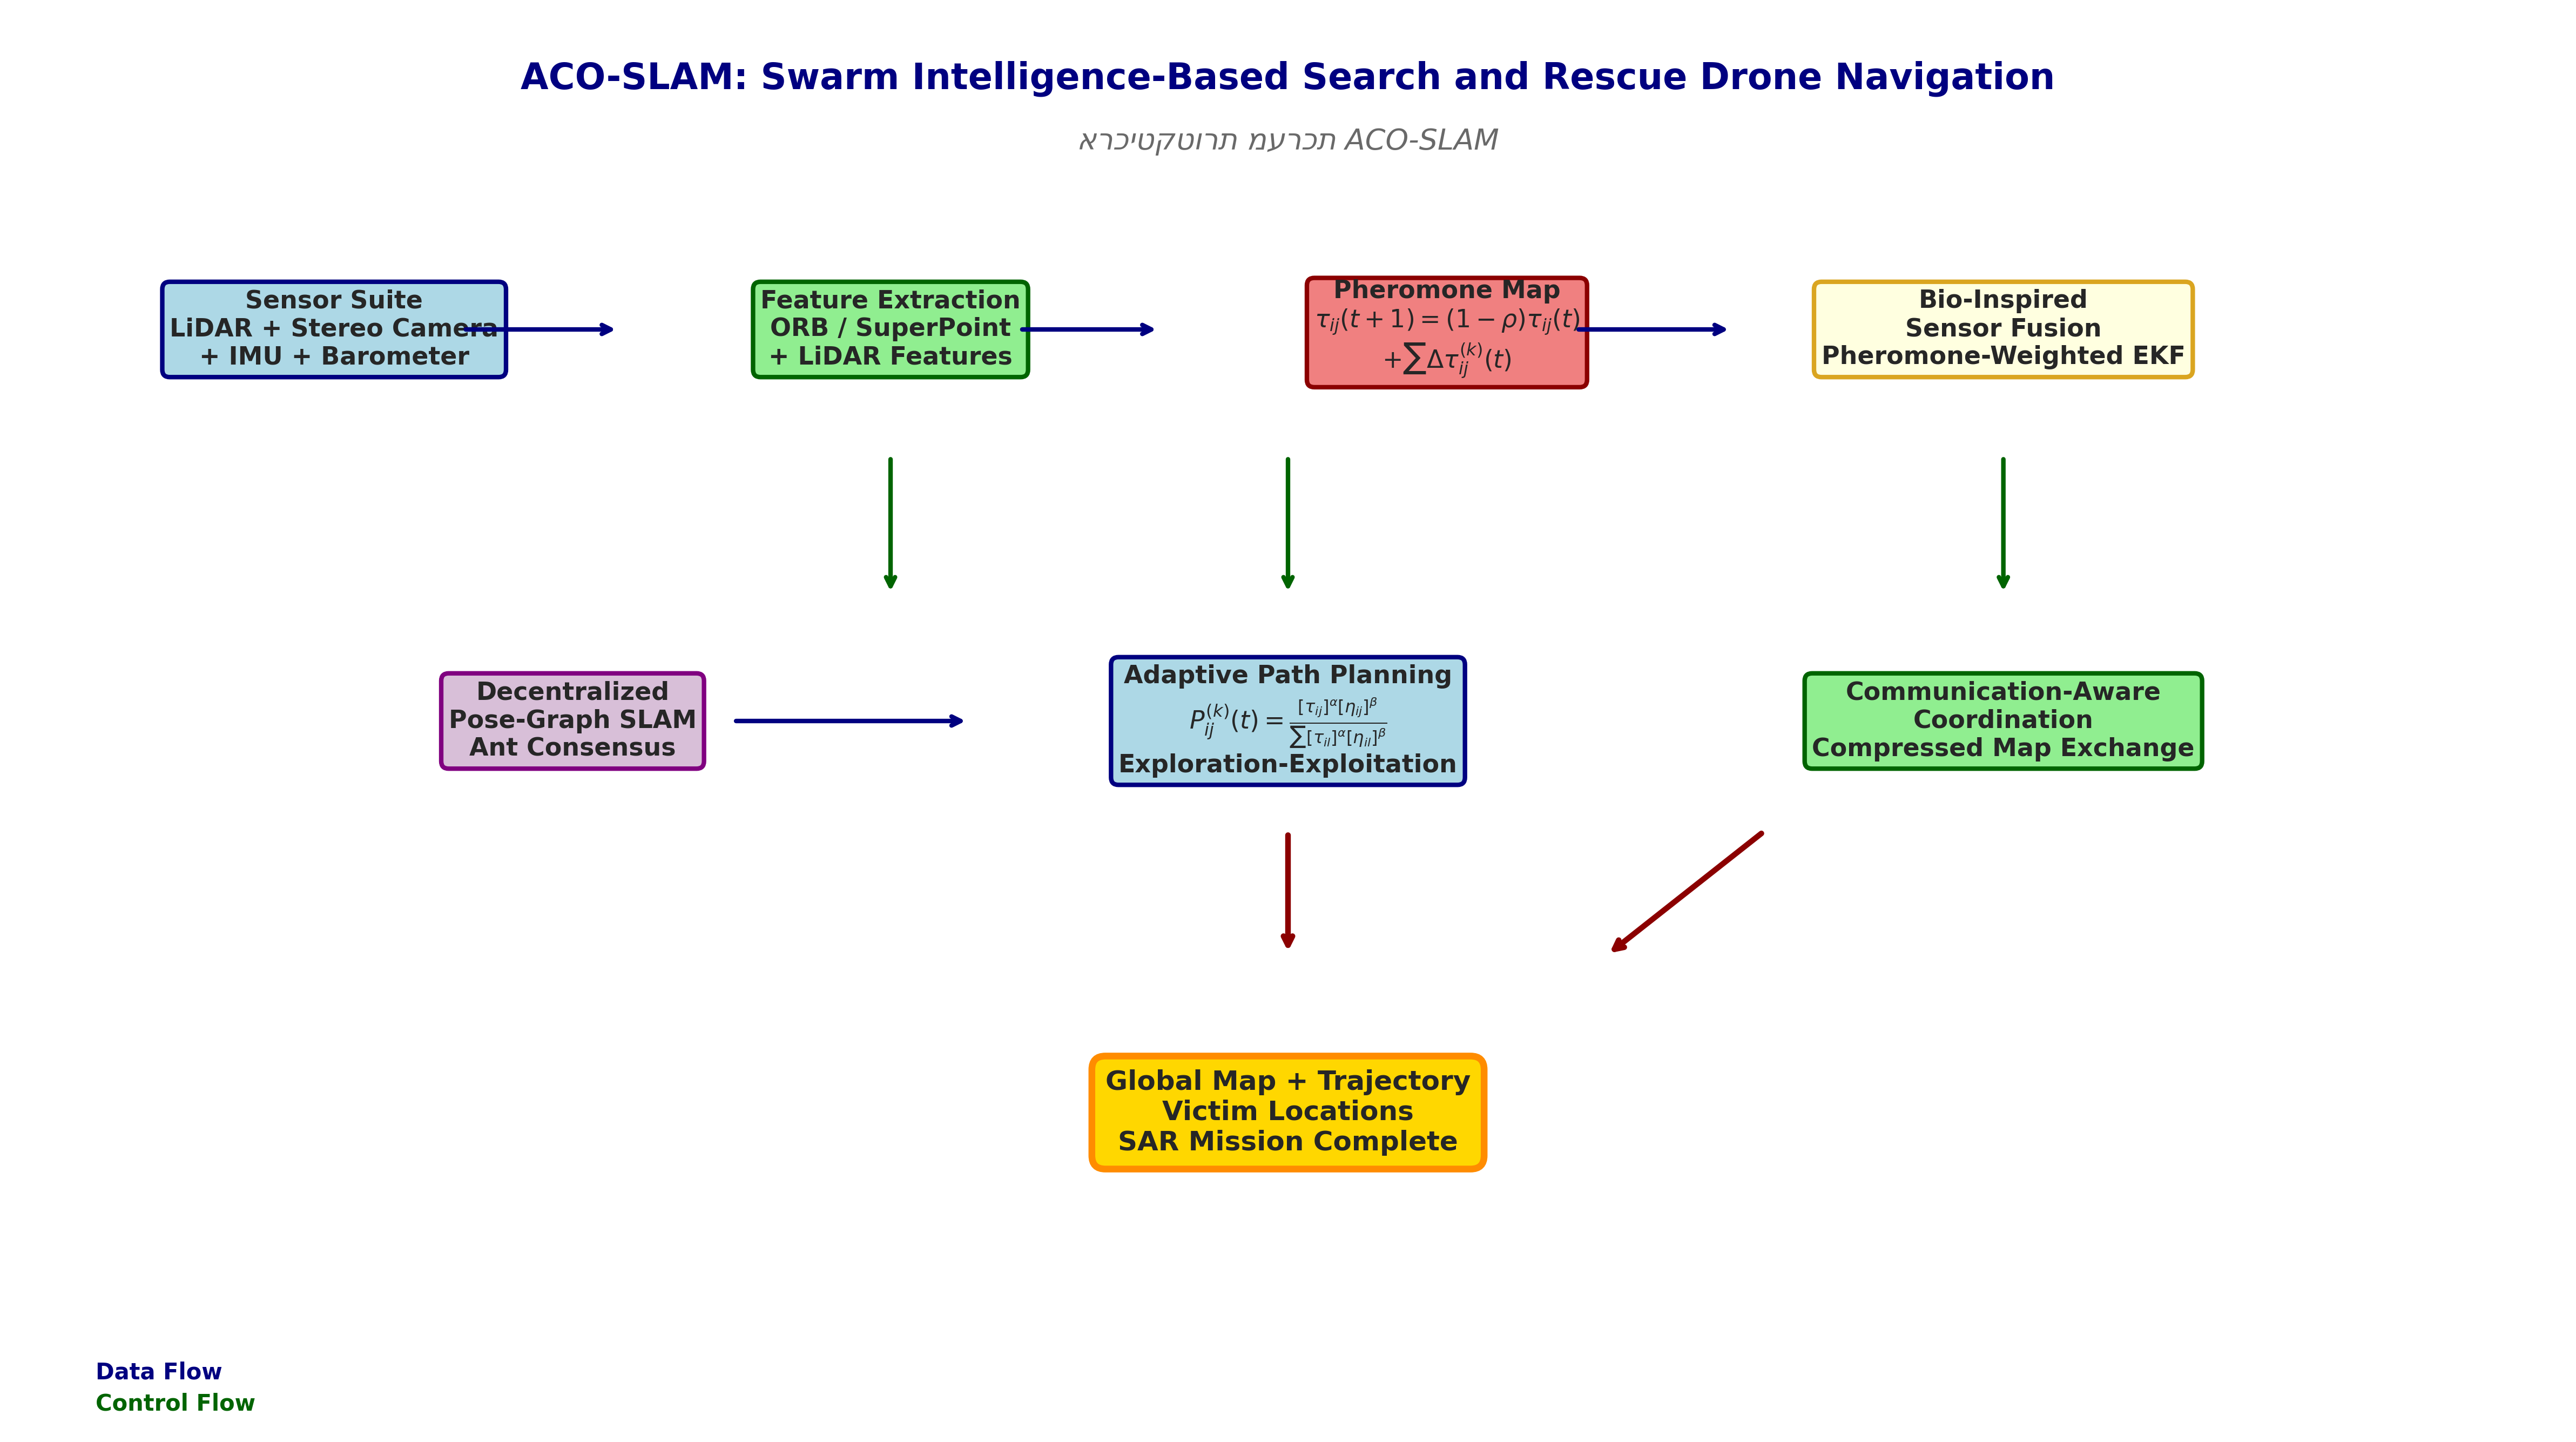
\includegraphics[width=0.98\columnwidth]{figures/fig_ac_slam_architecture.png}
\caption{ארכיטקטורת מערכת \en{ACO-SLAM}: תרשים זרימה הכולל את מערך החיישנים, מיצוי תכונות, מפת פרומונים, מיזוג רב-מודאלי, \en{SLAM} מבוזר ותכנון מסלול אדפטיבי.}
\label{fig:ac_slam_architecture}
\end{figure}

\begin{table}[htbp]
\centering
\caption{השוואה בין שיטות \en{SLAM} להקתי קיימות לבין השיטה המוצעת \en{ACO-SLAM}.}
\label{tab:comparison_methods}
\adjustbox{max width=\columnwidth}{%
\begin{tabular}{lcccc}
\toprule
שיטה & מבוזר & פרומונים & אסטרטגיית חקר & מיזוג חיישנים \\
\midrule
\en{Swarm-SLAM} \cite{Lajoie2023SwarmSLAM} & $\checkmark$ & $\times$ & אקראי & \en{LiDAR}+מצלמה \\
\en{D2SLAM} \cite{Xu2024D2SLAM} & $\checkmark$ & $\times$ & חמדן & \en{Visual-Inertial} \\
\en{ORB-SLAM3} \cite{Campos2021ORBSLAM3} & $\times$ & $\times$ & \en{N/A} & \en{Visual-Inertial} \\
\en{ACO-SLAM} (מוצע) & $\checkmark$ & $\checkmark$ & אדפטיבי & רב-מודאלי מבוסס פרומונים \\
\bottomrule
\end{tabular}%
}
\end{table}

\subsection{מבנה המאמר}
\label{sec:paper_structure}

המאמר מאורגן כדלקמן: פרק 2 מציג את ניסוח הבעיה ומודל המערכת, כולל מודל הרחפן והחיישנים, מודל הסביבה, מודל התקשורת והגדרת בעיית ה-\en{SLAM} השיתופי. פרק 3 מתאר את אופטימיזציית מושבת הנמלים לחקר להקתי, תוך התמקדות בעקרונות \en{ACO} קלאסיים, התאמתם לחקר רב-רחפנים, פונקציית ההתאמה לחקר \en{SAR} והאלגוריתם המוצע. פרק 4 מציג את מיזוג החיישנים הרב-מודאלי בהשראה ביולוגית, כולל מודל החיישנים, מיזוג מבוסס נמלים והתמודדות עם רעש ואובדן חיישנים. פרק 5 מתאר את ה-\en{SLAM} המבוזר מבוסס גרף תנוחות עם קונצנזוס נמלים, כולל זיהוי לולאות סגירה מבוסס פרומון ואופטימיזציית גרף מבוזרת. פרק 6 מציג את תכנון המסלול האדפטיבי לחיפוש והצלה, כולל מודל דינמיקת החיפוש, איזון חקר-ניצול והימנעות מהתנגשויות. פרק 7 דן בתיאום מודע תקשורת, כולל העברת מפות פרומונים דחוסה ואסטרטגיית רחפן-שליח. פרק 8 מציג תוצאות סימולציה וניסויים מקיפים, כולל השוואת ביצועי \en{SLAM}, ביצועי חיפוש והצלה וניתוח רגישות פרמטרים. פרק 9 מסכם את המאמר, דן במגבלותיו ומציע כיווני מחקר עתידיים.

לסיכום, פרק מבוא זה הציג את הרקע והמוטיבציה לחקר ניווט להקות רחפנים למשימות חיפוש והצלה, הגדיר את הבעיה הפורמלית, הציג את ארבע התרומות המרכזיות של המאמר, סקר את הספרות הרלוונטית, השווה את הגישה המוצעת לשיטות קיימות ותיאר את מבנהו. הפרק הבא יפרט את ניסוח הבעיה המלא ואת מודל המערכת.

\cite{Lajoie2023SwarmSLAM, Xu2024D2SLAM, Dorigo2004ACO, Schroder2007ACO, Campos2021ORBSLAM3, Qin2018VINSMono, Zhang2014LOAM, Schnitzler1968DSC, Waharte2010SAR, Perez2018MultiUAV, Choudhary2017Comm, Dutta2020CommSLAM}
